\chapter{Manuel d'utilisation}

\section{Menu du jeu}

\subsection{Menu principal}

Au lancement du jeu le menu principal apparaît. La figure
\ref{fig:manuel-menu-principal} montre une copie d'écran du menu.
Le menu est composé de quatre boutons.

\begin{figure}[h]
    \centering
    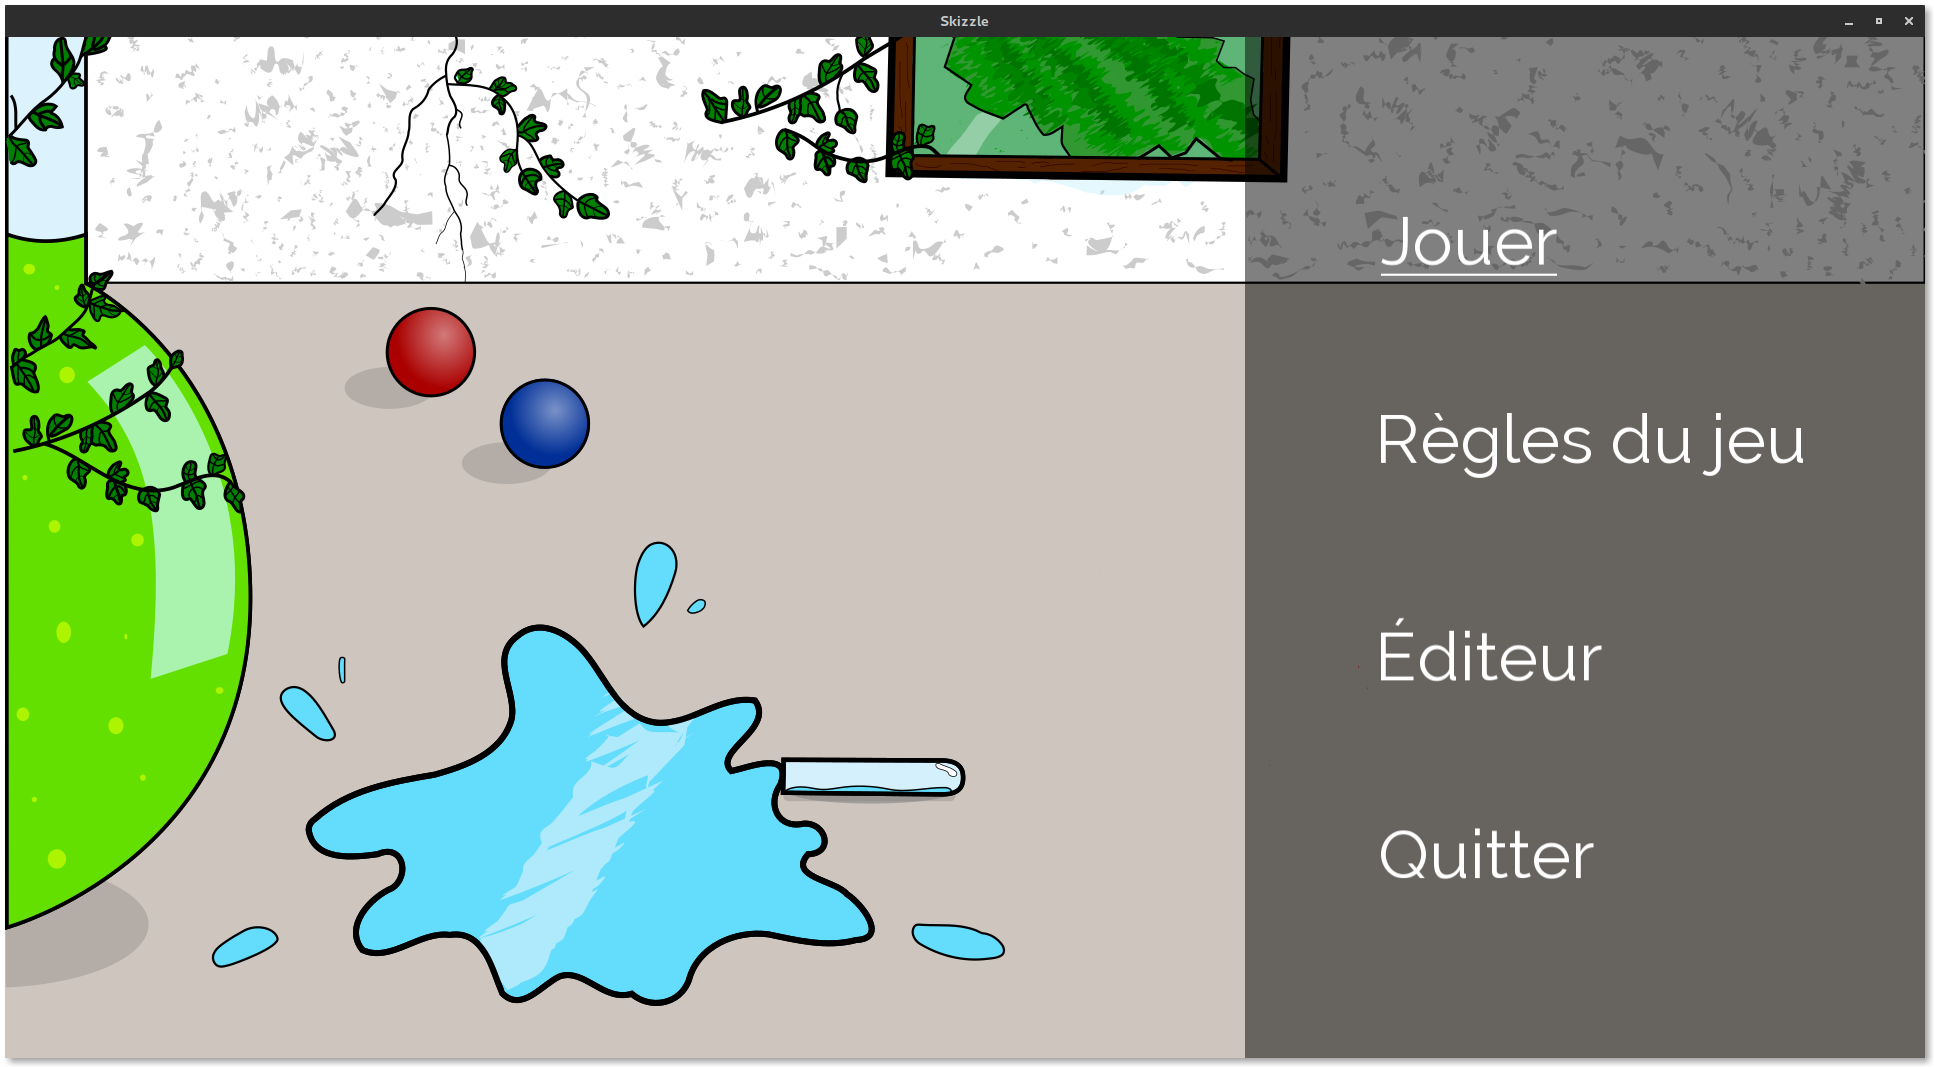
\includegraphics[width=13cm]{figures/manuel-menu-principal.png}
    \caption{Menu principal}
    \label{fig:manuel-menu-principal}
\end{figure}

\begin{description}
\item[Bouton jouer]
    Il permet d'accéder au menu de sélection des niveaux.
\item[Bouton règles du jeu]
    Il démarre la vue affichant les règles du jeu.
\item[Bouton éditeur]
    Il permet d'accéder au menu permettant de créer un niveau
    ou d'en éditer un existant.
\item[Bouton quitter]
    Il quitte le jeu.
\end{description}

\subsection{Menu de sélection du niveau}

\begin{figure}[h]
    \centering
    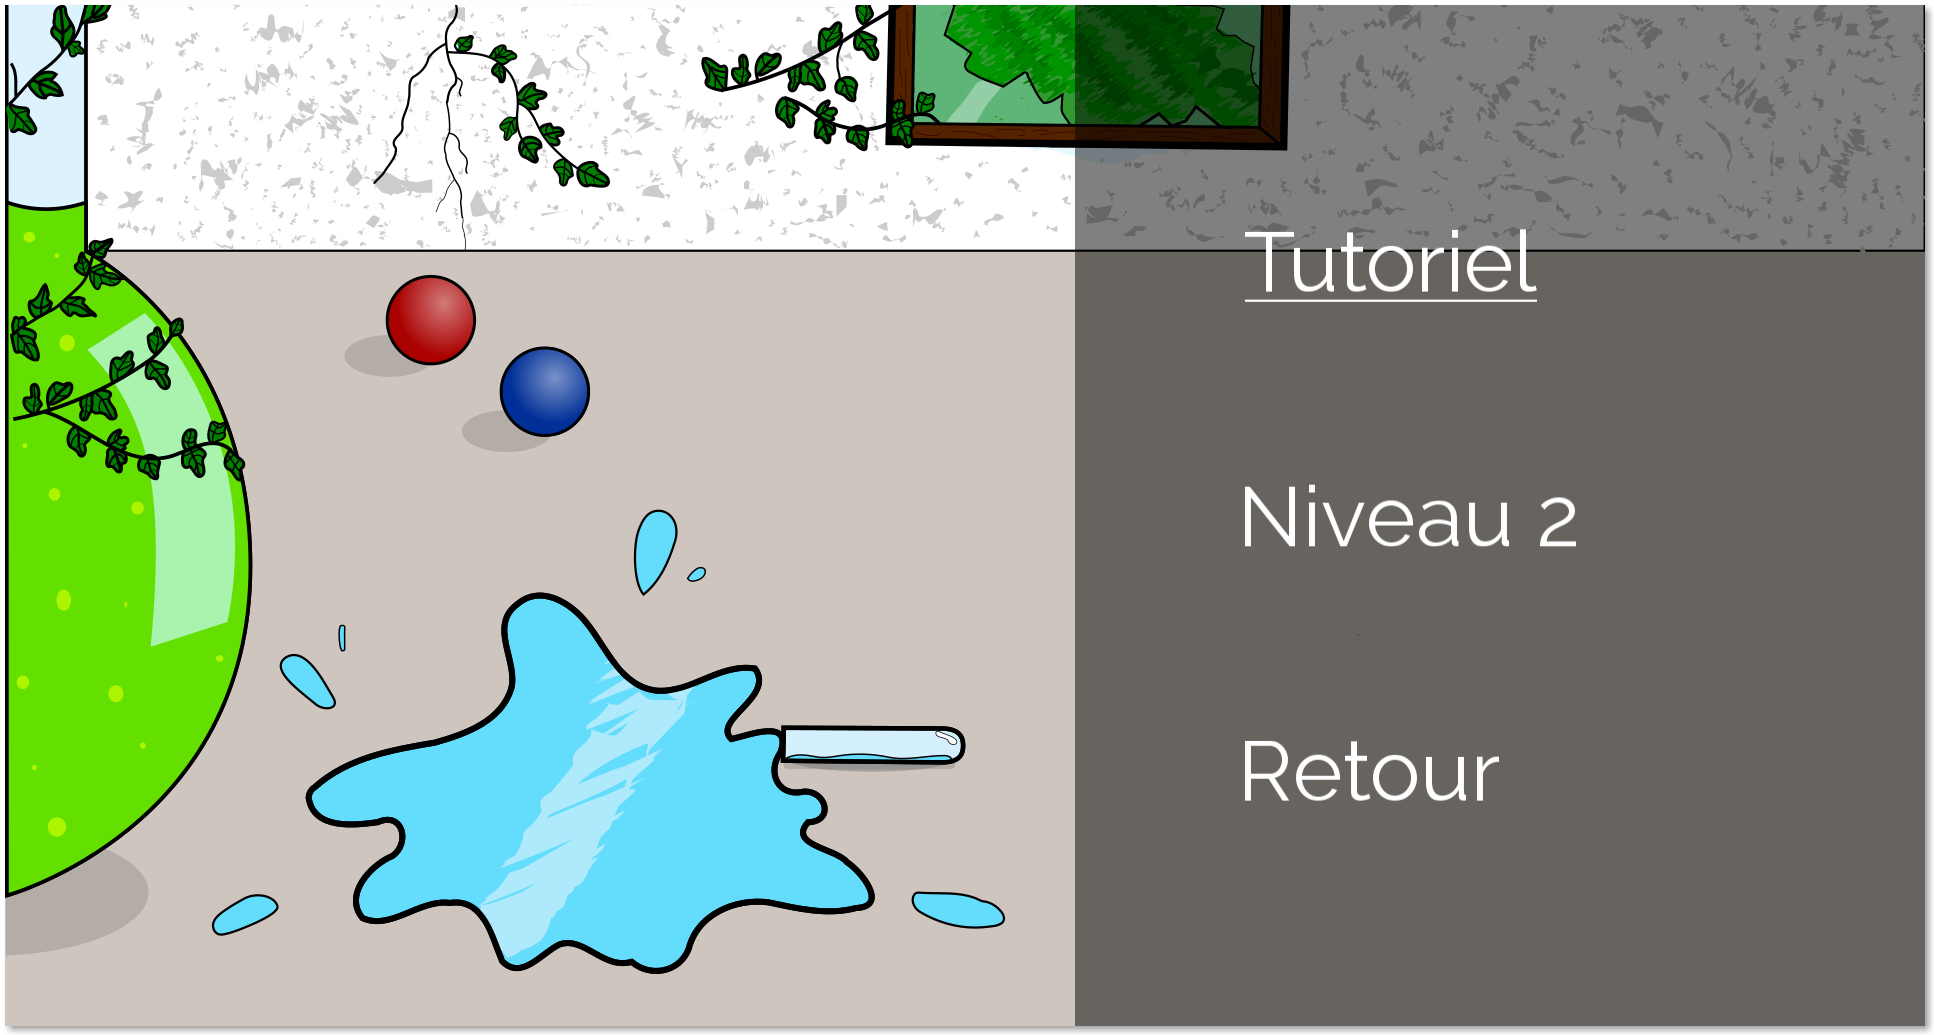
\includegraphics[width=13cm]{figures/manuel-menu-jouer.png}
    \caption{Menu de sélection du niveau}
    \label{fig:manuel-menu-selection}
\end{figure}

Le menu de sélection des niveaux, dont une copie d'écran est présentée
en figure \ref{fig:manuel-menu-selection}, se compose de deux types de boutons.
Les boutons niveaux permettent au joueur de choisir un niveau à jouer et
le bouton retour pour revenir vers le menu principal.

\subsection{Menu de l'éditeur}

\begin{figure} [!h]
    \centering
    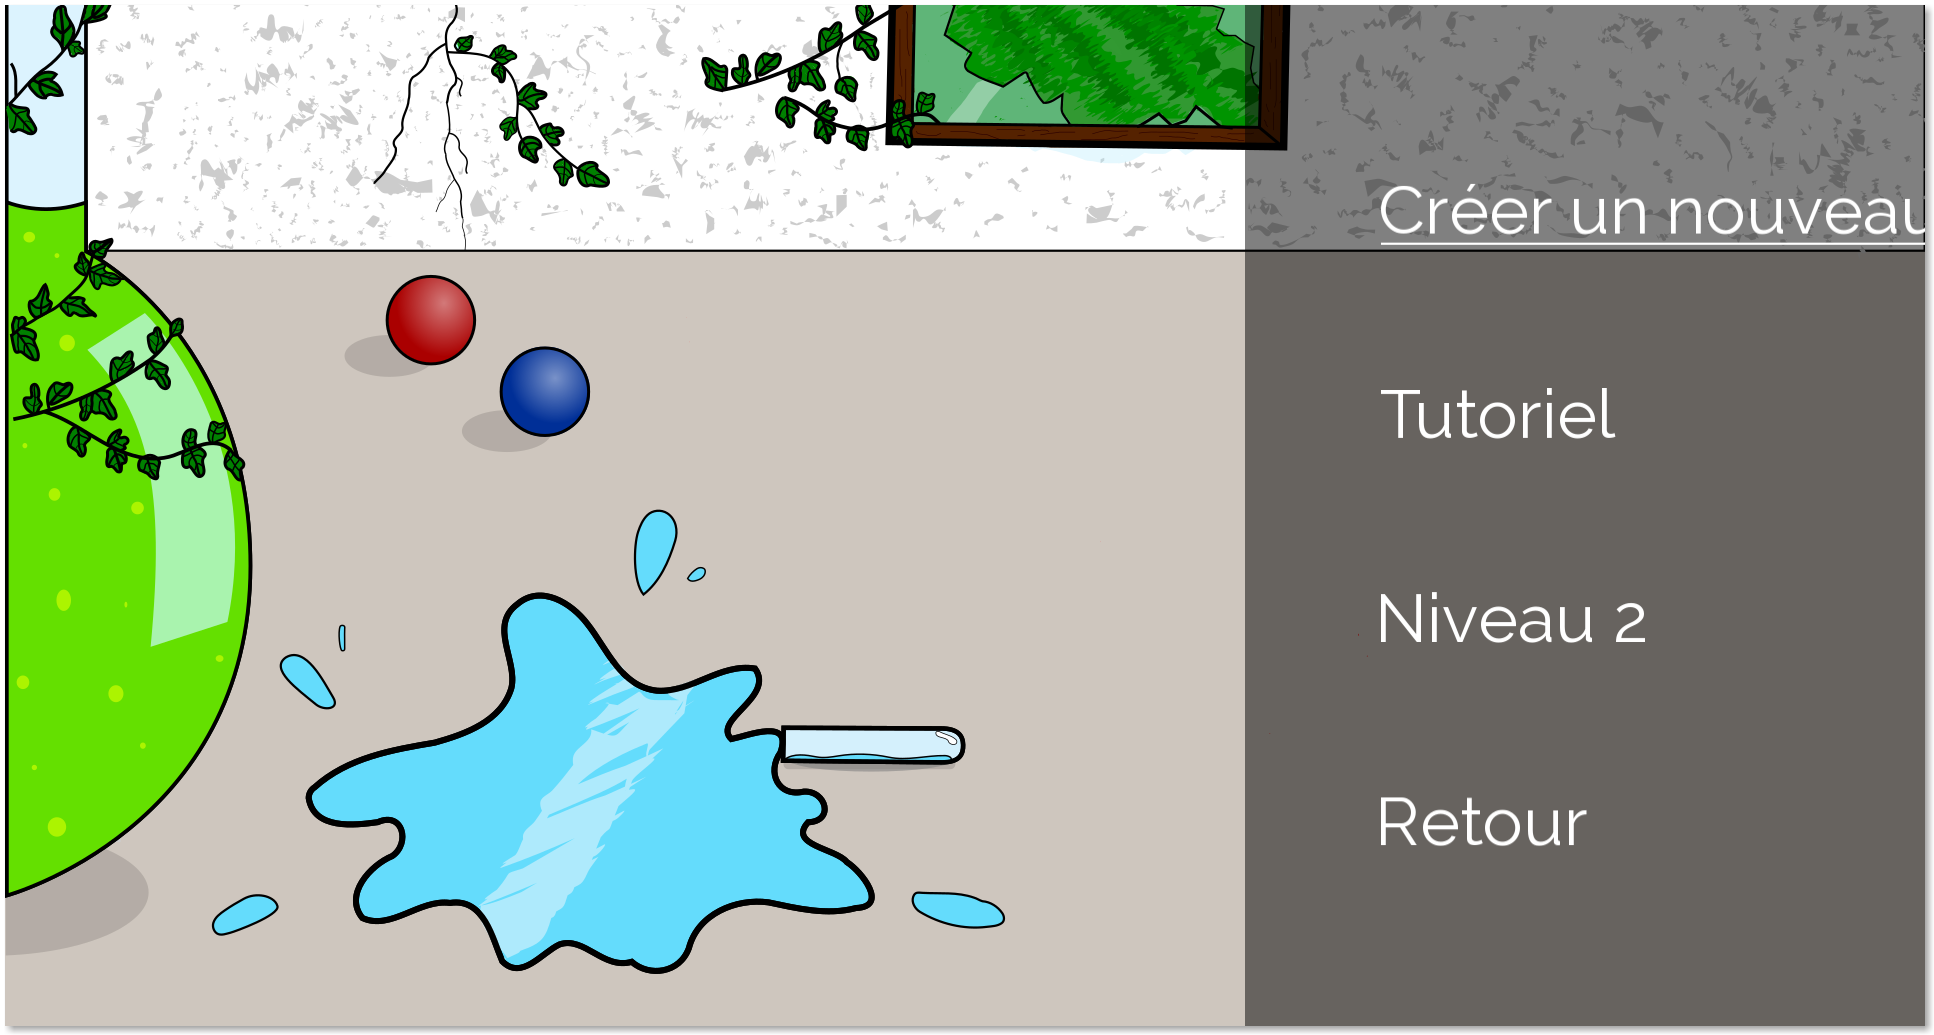
\includegraphics[width=13cm]{figures/manuel-menu-editeur.png}
    \caption{Menu de l'éditeur}
    \label{fig:manuel-menu-editeur}
\end{figure}

Le menu de l'éditeur, dont une copie d'écan est présentée en figure
\ref{fig:manuel-menu-editeur}, se compose de trois types de boutons.
Créer un nouveau niveau pour démarrer la création d'un niveau à partir
de rien, éditer un niveau déjà existant, et retour qui renvoie vers
le menu principal.

Dans les menus, les touches \fbox{$\uparrow$}, \fbox{$\downarrow$} ou
le passage de la souris sur un des boutons permettent de séléctionner un
élément du menu. Le bouton actuellement sélectionné est souligné.

La touche \fbox{Entrée} ou un clic avec la souris permettent de valider le choix.

Les touches \fbox{$\longleftarrow$} et \fbox{Échap} permettent de revenir
au menu précédent.

\section{Objets}
\label{sec:manuel-objets}
\newcommand{\objectsymbol}[1]{
    \includegraphics[width=23px]{figures/manuel-#1.png}
}

\newcommand{\describeobject}[2]{
    \noindent
    \begin{minipage}{.08\textwidth}
        \objectsymbol{#1}
    \end{minipage}
    \begin{minipage}{.9\textwidth}
        #2
    \end{minipage}
}

Les niveaux se composent d'une collection d'objets qui
interagissent entre eux par les lois physiques ou par
l'action du joueur, selon les types d'entités. Nous
définissons dans cette section les comportements
des différents objets.

\subsection{Balles}

\describeobject{ball}{
    Les balles sont des objets controlés par les joueurs. Chaque joueur
    est affecté à une balle, identifiée de manière unique par son numéro.
}

\subsubsection{Polarité}

\describeobject{charge-neg}{
    Les objets de couleur bleue repoussent tous ceux de la même couleur
    et attirent les objets de couleur rouge.
}

\describeobject{charge-pos}{
    Les objets de couleur rouge repoussent tous ceux de la même couleur
    et attirent les objets de couleur bleue.
}

\subsubsection{Blocs}

\describeobject{block}{
    Le bloc de base ne réalise aucune action particulière, il sert
    uniquement à délimiter des zones dans le niveau.
}

\describeobject{movable-block}{
    La caisse est un bloc qui peut être déplacé par les joueurs
    ou une autre caisse. Elle active les blocs de gravité comme les joueurs.
}

\describeobject{gravity-block}{
    Le bloc de gravité modifie le sens de la gravité du niveau lorsqu'un joueur
    ou une caisse l'active en rentrant en collision avec lui. Ce bloc n'est
    activable qu'une seule fois par partie.
}

\describeobject{switch-block}{
    Le bloc inverseur inverse la charge des balles qui l'activent
    en rentrant en collision avec lui. Ce bloc n'est activable qu'une
    seule fois par partie.
}

\describeobject{kill-block}{
    Le bloc tueur fait perdre la partie si un des deux joueurs l'active en
    rentrant en collision avec lui.
}

\describeobject{finish-block}{
    Le bloc d'arrivée fait gagner la partie lorsque tous les joueurs
    l'ont activé en rentrant en collision avec lui.
}

\section{Jeu}

Les joueurs ne peuvent déplacer leurs balles que vers la gauche ou la droite.
Le joueur 1 utilise \fbox{$\rightarrow$} pour se déplacer vers la droite et
\fbox{$\leftarrow$} pour se déplacer vers la gauche. Le joueur 2 utilise
\fbox{D} pour se déplacer vers la droite et \fbox{Q} pour se déplacer
vers la gauche.

Les joueurs peuvent mettre le jeu en pause avec la touche \fbox{Échap},
ou bien quitter le niveau en appuyant sur \fbox{Espace}.

La partie peut être perdue pour trois raisons~: si un joueurs a
activée un bloc tueur, si un joueur est sortie de la zone de jeu
ou si le temps s'est écoulé totalement.

\section{Éditeur}

\subsection{Gestion des objets}

La figure \ref{fig:manuel-editeur-example} montre un exemple de niveau
en édition dans l'éditeur. On peut sélectionner le type d'objet à placer
en cliquant à la souris dans la barre latérale droite.

Un clic gauche sur une zone libre permet de placer le type d'objet
actuellement sélectionné. Le maintien du clic gauche en déplaçant la
souris permet de placer plusieurs objets à la fois.

\begin{figure}[h]
    \centering
    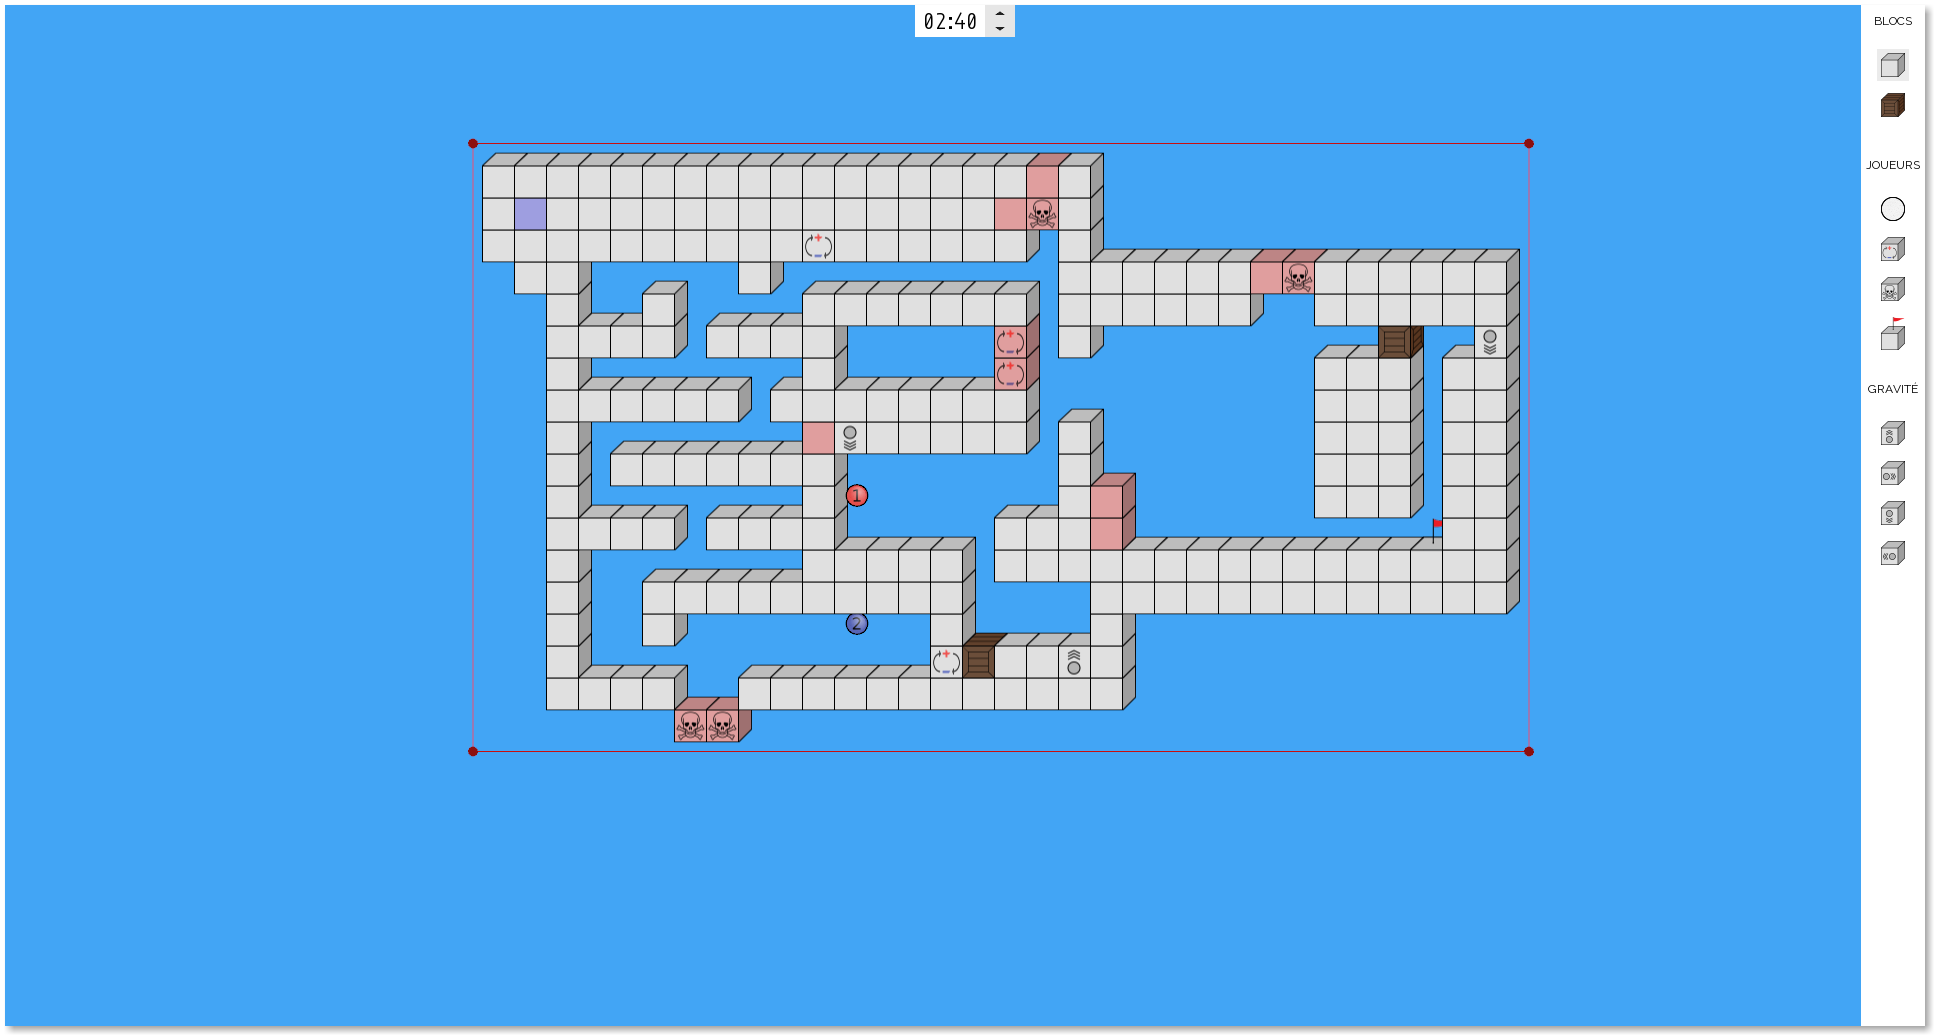
\includegraphics[width=13cm]{figures/manuel-editor.png}
    \caption{Exemple de niveau en cours d'édition dans l'éditeur}
    \label{fig:manuel-editeur-example}
\end{figure}

Pour modifier la charge d'un objet, le curseur doit être placé sur
celui-ci. La touche \fbox{Ctrl} doit être enfoncée tout en faisant
glisser la mollette de la souris, ou bien en faisant glisser deux
doigts sur le pavé tactile vers le haut ou le bas. L'objet change
de couleur en conséquence.

La sélection d'un objet se fait en cliquant sur celui-ci. Pour sélectionner
plusieurs objets, on maintient \fbox{Ctrl} et on clique sur les objets.
On peut effectuer une sélection rectangulaire en maintenant la touche
\fbox{Shift} et en faisant glisser la souris sur la zone à sélectionner,
en maintenant le clic gauche enfoncé. Lorsqu'un objet est sélectionné, sa
bordure devient rouge, comme montré dans la figure \ref{fig:manuel-selection}.

\begin{figure}[h]
    \centering
    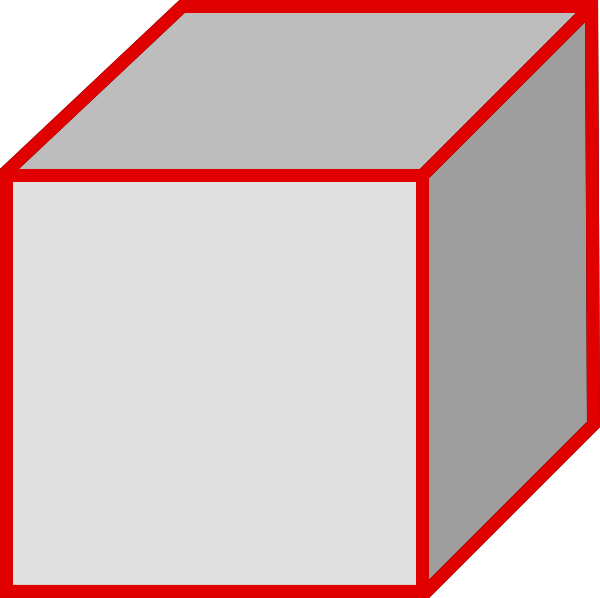
\includegraphics[width=25px]{figures/manuel-selected-block.png}
    \caption{Exemple d'objet sélectionné}
    \label{fig:manuel-selection}
\end{figure}

La suppression d'un objet s'effectue en cliquant dessus avec le bouton
droit de la souris. Pour supprimer tous les objets actuellement sélectionnés,
il suffit d'appuyer sur la touche \fbox{Suppr}.

\subsection{Compte à rebours}

Le compte à rebours se situe en haut au centre de le fenêtre. Durant la partie,
s'il arrive à 0, les joueurs meurent et la partie est perdue.

La valeur du compte à rebours peut être modifiée dans l'éditeur en cliquant
sur les flèches se situant à coté, ou en glissant la molette en gardant la
souris sur le compteur.

\subsection{Zone de jeu}

La zone jouable est représentée dans l'éditeur par un polygone
rouge composé de quatre points. Chacun de ces points peuvent être
déplacés en cliquant dessus afin de modifier la taille et la
forme de la zone.

\subsection{Gestion de la caméra}

Le déplacement de la caméra s'effectue en déplaçant la souris vers
une bordure de la fenêtre. La molette de la souris peut être utilisée
pour un défilement vertical, ou horizontal si la touche \fbox{Shift}
est enfoncée.

\subsection{Commandes générales}

Il est possible de tester le niveau à tout moment en appuyant sur la
touche \fbox{Espace}. Pour revenir à l'édition il suffit d'appuyer à
nouveau sur \fbox{Espace}.

Afin de sauvegarder le niveau il est nécessaire de réaliser la
combinaison de touches suivantes : \fbox{Ctrl} + \fbox{S}. (en mode édition).
Si vous ne sauvegardez pas vos changements, ils seront perdus.

Pour quitter l’éditeur et revenir au menu la touche \fbox{Échap} doit être utilisée.
